% Options for packages loaded elsewhere
\PassOptionsToPackage{unicode}{hyperref}
\PassOptionsToPackage{hyphens}{url}
%
\documentclass[
  12pt,
]{article}
\usepackage{amsmath,amssymb}
\usepackage{setspace}
\usepackage{iftex}
\ifPDFTeX
  \usepackage[T1]{fontenc}
  \usepackage[utf8]{inputenc}
  \usepackage{textcomp} % provide euro and other symbols
\else % if luatex or xetex
  \usepackage{unicode-math} % this also loads fontspec
  \defaultfontfeatures{Scale=MatchLowercase}
  \defaultfontfeatures[\rmfamily]{Ligatures=TeX,Scale=1}
\fi
\usepackage{lmodern}
\ifPDFTeX\else
  % xetex/luatex font selection
  \setmainfont[]{Times New Roman}
\fi
% Use upquote if available, for straight quotes in verbatim environments
\IfFileExists{upquote.sty}{\usepackage{upquote}}{}
\IfFileExists{microtype.sty}{% use microtype if available
  \usepackage[]{microtype}
  \UseMicrotypeSet[protrusion]{basicmath} % disable protrusion for tt fonts
}{}
\makeatletter
\@ifundefined{KOMAClassName}{% if non-KOMA class
  \IfFileExists{parskip.sty}{%
    \usepackage{parskip}
  }{% else
    \setlength{\parindent}{0pt}
    \setlength{\parskip}{6pt plus 2pt minus 1pt}}
}{% if KOMA class
  \KOMAoptions{parskip=half}}
\makeatother
\usepackage{xcolor}
\usepackage[margin=1in]{geometry}
\usepackage{graphicx}
\makeatletter
\def\maxwidth{\ifdim\Gin@nat@width>\linewidth\linewidth\else\Gin@nat@width\fi}
\def\maxheight{\ifdim\Gin@nat@height>\textheight\textheight\else\Gin@nat@height\fi}
\makeatother
% Scale images if necessary, so that they will not overflow the page
% margins by default, and it is still possible to overwrite the defaults
% using explicit options in \includegraphics[width, height, ...]{}
\setkeys{Gin}{width=\maxwidth,height=\maxheight,keepaspectratio}
% Set default figure placement to htbp
\makeatletter
\def\fps@figure{htbp}
\makeatother
\setlength{\emergencystretch}{3em} % prevent overfull lines
\providecommand{\tightlist}{%
  \setlength{\itemsep}{0pt}\setlength{\parskip}{0pt}}
\setcounter{secnumdepth}{-\maxdimen} % remove section numbering
\usepackage{booktabs}
\usepackage{longtable}
\usepackage{array}
\usepackage{multirow}
\usepackage{wrapfig}
\usepackage{float}
\usepackage{colortbl}
\usepackage{pdflscape}
\usepackage{tabu}
\usepackage{threeparttable}
\usepackage{threeparttablex}
\usepackage[normalem]{ulem}
\usepackage{makecell}
\usepackage{xcolor}
\ifLuaTeX
  \usepackage{selnolig}  % disable illegal ligatures
\fi
\usepackage{bookmark}
\IfFileExists{xurl.sty}{\usepackage{xurl}}{} % add URL line breaks if available
\urlstyle{same}
\hypersetup{
  pdftitle={Assessing the Impact of Airbnb's Plus Program: A Fixed Effects Analysis with Cross-Sectional and Time-Series Dimensions},
  pdfauthor={Amir Eid, Leander Tim Engel, Aurel Roedern and Federico Scandizzo},
  hidelinks,
  pdfcreator={LaTeX via pandoc}}

\title{Assessing the Impact of Airbnb's Plus Program: A Fixed Effects
Analysis with Cross-Sectional and Time-Series Dimensions}
\author{Amir Eid, Leander Tim Engel, Aurel Roedern and Federico
Scandizzo}
\date{}

\begin{document}
\maketitle

\setstretch{1.5}
\section{Introduction}\label{introduction}

This study builds on prior research exploring the Airbnb Plus program's
impact on \textbf{booking\_rate}, which found no significant effect.
Addressing limitations such as unobserved factors and missing fixed
effects, it uses a Fixed Effects model to estimate the program's causal
effect by comparing treated cities (Nashville, New Orleans, Washington
DC, Denver) to controls, accounting for \textbf{employment\_rate},
\textbf{price\_mean}, and \textbf{year\_built\_to\_now}. Additionally,
the study examines the impact of the program on
\textbf{listing\_avg\_review}, testing whether it increases customer
satisfaction in treated cities compared to controls, after controlling
for city-specific and time-specific effects.

\section{1. Refining Hypotheses}\label{refining-hypotheses}

The \textbf{first hypothesis} is, therefore, the following:

\begin{itemize}
\item
  \(H_0:\) The introduction of the Airbnb Plus program does not
  significantly affect booking rates in treated cities compared to
  control cities, after accounting for city-specific and time-specific
  effects (i.e., \emph{β3 = 0}, where β3 is the coefficient of the
  interaction term).
\item
  \(H_a:\) The introduction of the Airbnb Plus program does
  significantly affect booking rates in treated cities compared to
  control cities, after accounting for city-specific and time-specific
  effects (i.e.,\emph{β3 ≠ 0}). \[
  \text{booking\_rate}_{it} = \alpha_i + \gamma_t + \beta_3 (Plus_i \times Treated_i) + \epsilon_{it}
  \] The \textbf{second hypothesis} is formulated as follows:
\item
  \(H_0:\) The introduction of the Airbnb Plus program does not increase
  listing average reviews in treated cities compared to control cities,
  after accounting for city-specific and time-specific effects (i.e.,
  \emph{β3 ≤ 0}, where β3 is the coefficient of the interaction term).
\item
  \(H_a:\) The introduction of the Airbnb Plus program increases listing
  average reviews in treated cities compared to control cities, after
  accounting for city-specific and time-specific effects (i.e., \emph{β3
  \textgreater{} 0}). \[
  \text{listing\_avg\_review}_{it} = \alpha_i + \gamma_t + \beta_3 (Plus_i \times Treated_i) + \epsilon_{it}
  \] Where:
\item
  \textbf{\(\alpha_i\)}: City fixed effects
\item
  \textbf{\(\gamma_t\)}: Time fixed effects, affecting all cities
  equally
\item
  \textbf{group}: Indicator variable for whether cities are in the
  \textbf{treated} or \textbf{control} group
\item
  \textbf{\(\beta_3 (\text{Plus} \times \text{Treated})\)}: Interaction
  term capturing the DiD effect
\item
  \(\epsilon_{it}\): Error term, capturing random noise or unobserved
  factors varying across cities and over time
\end{itemize}

\section{2. Dataset Overview, Data Quality \& Model-Free
Investigation}\label{dataset-overview-data-quality-model-free-investigation}

As the Airbnb Plus program is implemented in five cities, five others
will serve as controls. San Francisco, part of the pilot phase, is
excluded to avoid bias. The dataset includes 14604 observations across
99 variables, covering 773 zip codes in 11 U.S. cities from August 2017
(\texttt{timeperiod} = 8) to October 2019 (\texttt{timeperiod} = 34).
Key variables include \textbf{performance metrics}
(\texttt{booking\_rate}, \texttt{listing\_avg\_reviews}) and
\textbf{secondary variables} (\texttt{zipcode}, \texttt{timeperiod},
\texttt{city\_number}, \texttt{policy\_entry},
\texttt{employment\_rate}, \texttt{price\_mean},
\texttt{year\_built\_to\_now}). Additional variables created for
analysis are:\\
- \textbf{\texttt{city\_name}}: maps \texttt{city\_number} to city names
or \emph{Others}.\\
- \textbf{\texttt{date}}: converts \texttt{timeperiod} to year-month
format.\\
- \textbf{\texttt{group}}: distinguishes treated and control cities.\\
- \textbf{\texttt{time}}: flags pre- and post-Plus program periods.

To begin assessing the quality of the data-set, the following shows a
quick inspection, showing the structure of the data.

\begingroup\fontsize{6}{8}\selectfont

\begin{longtable}[t]{rrrlrlrrrrr}
\caption{\label{tab:unnamed-chunk-3}Preview of the data}\\
\toprule
booking\_rate & zipcode & timeperiod & date & city\_number & city\_name & policy\_entry & employment\_rate & price\_mean & listing\_avg\_review & year\_built\_to\_now\\
\midrule
NA & 1217 & 23 & 2018-11-01 & 1 & Others & 0 & NA & 132.5000 & -1 & NA\\
0.7500000 & 1217 & 24 & 2018-12-01 & 1 & Others & 0 & NA & 158.0000 & -1 & NA\\
NA & 1217 & 25 & 2019-01-01 & 1 & Others & 0 & NA & 179.5000 & -1 & NA\\
-0.1250000 & 1217 & 26 & 2019-02-01 & 1 & Others & 0 & NA & 212.0000 & -1 & NA\\
0.8666667 & 1217 & 27 & 2019-03-01 & 1 & Others & 0 & NA & 207.3333 & -1 & NA\\
\addlinespace
NA & 1217 & 28 & 2019-04-01 & 1 & Others & 0 & NA & 207.0000 & -1 & NA\\
\bottomrule
\end{longtable}
\endgroup{}

\subsubsection{Missing Values}\label{missing-values}

During the data cleaning process, a total of 1760 missing values were
identified across various variables, including \textbf{booking\_rate},
\textbf{employment\_rate}, \textbf{price\_mean},
\textbf{listing\_avg\_review}, \textbf{year\_built\_to\_now}. For
\textbf{booking\_rate}, both zero and negative values were retained, as
the variable reflects the ratio of bookings (positive values) to
cancellations (negative values). For \textbf{listing\_avg\_review},
negative values (-1) were treated as an indicator for a booking having
no reviews yet due to being new. These were treated as non-random
missing values. For this reason, instead of being replaced with the
mean, they were dropped to not introduce bias to the research. Instead,
actual missing values were treated as random ones and were replace with
the mean of the city. Similarly, for \textbf{price\_mean}, zeroes were
found and were dropped as these were likely input because there were no
listing prices in that specific zip code to compute the price mean. The
other variables did not have any zeroes or negative values, their actual
missing values were treated as random missing data and replaced with
their city mean. This approach was chosen to prevent the removal of
rows, which could have introduced gaps in time for certain zip codes and
cities. By using city-specific means, we minimized bias and retained as
much relevant data as possible.

Each variable was carefully examined, and it was found that most missing
values were NAs (rather than NaN or zeros). The imputation strategy
allowed for the preservation of data integrity, ensuring minimal
disruption to the overall data set. The cleaned data was then
summarized, confirming the successful handling of missing values and
providing a solid foundation for further analysis.

\subsubsection{Outliers}\label{outliers}

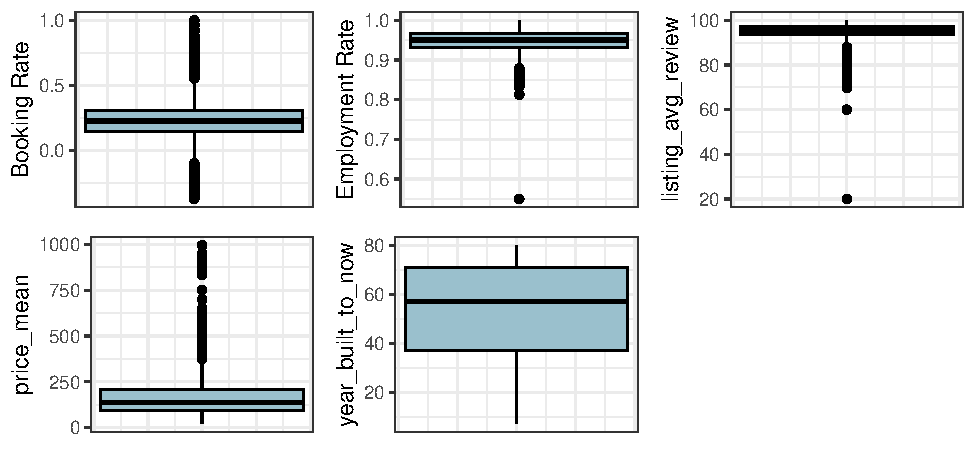
\includegraphics{assignment2_final_2_files/figure-latex/unnamed-chunk-6-1.pdf}
All variables show significant of outliers, except for
\textbf{year\_built\_to\_now}. \textbf{Listing\_avg\_review} and
\textbf{employment\_rate} outliers will be replaced with the mean for
their respective city number since they're likely caused by either a
very negative review or a random error, like an employment rate below
60\% for 11430 which is the zipcode for Queens County, NY. After a brief
online research, employment rates in this area were found to be unlikely
to drop below this threshold. Furthermore, listing average reviews and
booking rate will be truncated using 5th and 95th percentiles, retaining
only 90\% of the data which will be enough to test the hypotheses. Price
mean instead will be log-transformed to deal with its outliers.

\begin{table}[!htbp] \centering 
  \caption{Summary Statistics for Final Data Set} 
  \label{} 
\small 
\begin{tabular}{@{\extracolsep{5pt}}lcccccccc} 
\\[-1.8ex]\hline 
\hline \\[-1.8ex] 
Statistic & \multicolumn{1}{c}{N} & \multicolumn{1}{c}{Mean} & \multicolumn{1}{c}{St. Dev.} & \multicolumn{1}{c}{Min} & \multicolumn{1}{c}{Pctl(25)} & \multicolumn{1}{c}{Median} & \multicolumn{1}{c}{Pctl(75)} & \multicolumn{1}{c}{Max} \\ 
\hline \\[-1.8ex] 
booking\_rate & 10,702 & 0.230 & 0.105 & 0.000 & 0.159 & 0.228 & 0.300 & 0.473 \\ 
zipcode & 10,702 & 37,303.850 & 29,160.620 & 2,026 & 11,103 & 37,013 & 55,418 & 97,317 \\ 
timeperiod & 10,702 & 23.441 & 6.872 & 8 & 18 & 24 & 29 & 34 \\ 
city\_number & 10,702 & 6.964 & 2.688 & 1 & 6 & 7 & 10 & 11 \\ 
policy\_entry & 10,702 & 0.121 & 0.326 & 0 & 0 & 0 & 0 & 1 \\ 
employment\_rate & 10,702 & 0.944 & 0.030 & 0.813 & 0.930 & 0.950 & 0.965 & 1.000 \\ 
listing\_avg\_review & 10,702 & 95.317 & 2.114 & 90.500 & 93.727 & 95.218 & 97.000 & 99.833 \\ 
year\_built\_to\_now & 10,702 & 54.534 & 20.380 & 7.000 & 38.000 & 58.000 & 73.000 & 80.000 \\ 
log\_price\_mean & 10,702 & 4.969 & 0.484 & 3.624 & 4.573 & 4.937 & 5.332 & 6.745 \\ 
\hline \\[-1.8ex] 
\end{tabular} 
\end{table} 
\newpage

A panel data set was created for the DiD regression analysis, allowing
to compare changes before and after the introduction of the Airbnb Plus
program across multiple cities. The two dimensions of the data are
\textbf{city\_name} and \textbf{time}, where the former represents the
entities and the latter denotes the periods under study. The panel data
is balanced, meaning each city has data for all time periods.

\subsection{Model Free investigation}\label{model-free-investigation}

This section presents a model-free investigation using a
Difference-in-Differences (DiD) approach to assess the impact of Airbnb
Plus. We visualize booking rates and listing reviews before and after
the program's introduction for treated and control cities. This analysis
offers an intuitive understanding of the program's effects.

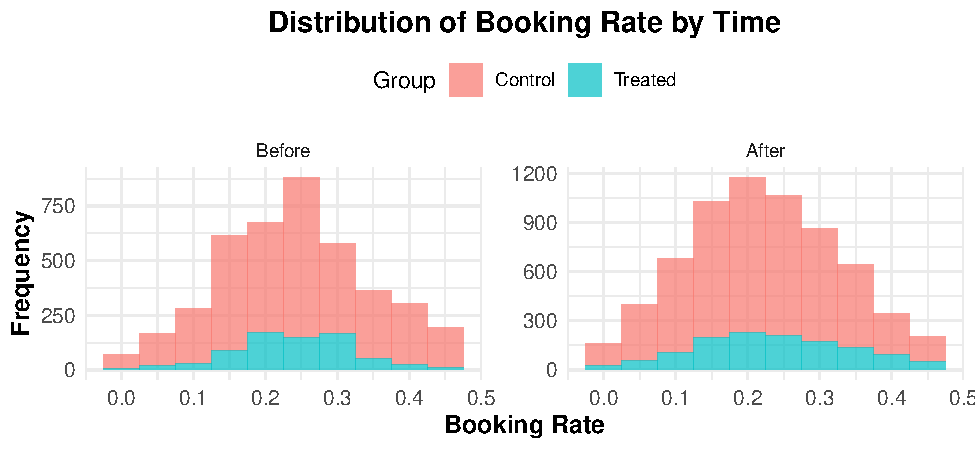
\includegraphics{assignment2_final_2_files/figure-latex/unnamed-chunk-12-1.pdf}
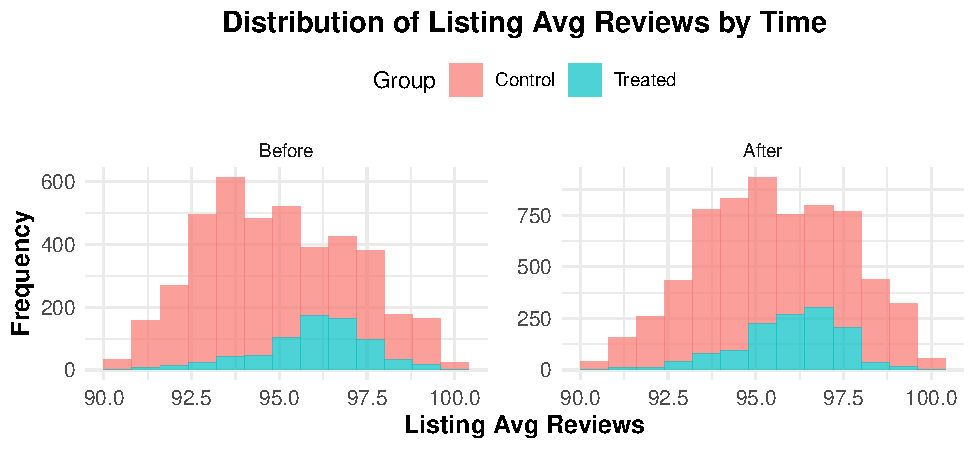
\includegraphics{assignment2_final_2_files/figure-latex/unnamed-chunk-12-2.pdf}

The distributions of \textbf{booking\_rate} and
\textbf{listing\_avg\_review} remain approximately normal before and
after implementing the program. Listing avg reviews appear to be
slightly left-skewed. In both cases, the control groups have more
observations than the treated group. The differences in group sizes may
lead to heteroscedasticity, impacting the precision of the interaction
term estimates.

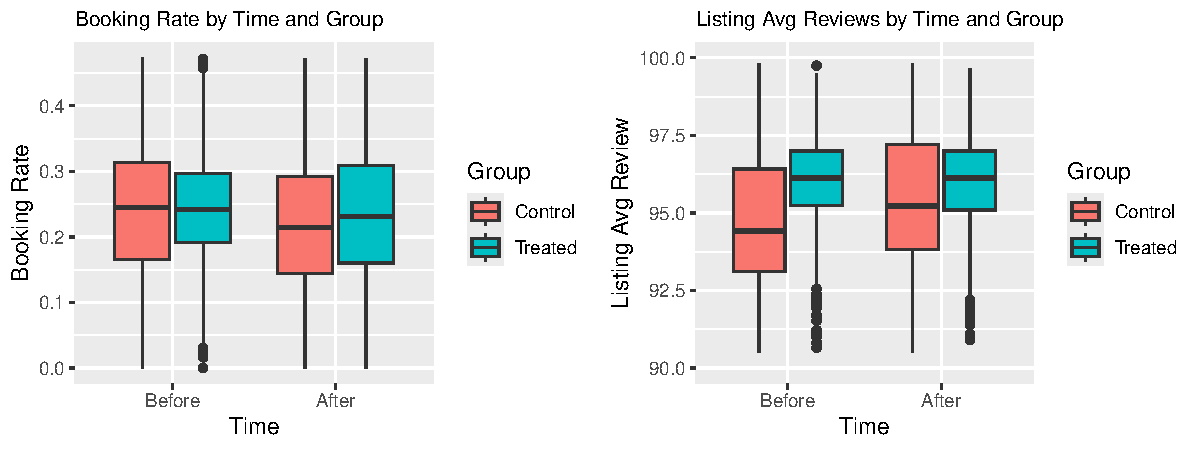
\includegraphics{assignment2_final_2_files/figure-latex/unnamed-chunk-14-1.pdf}

The boxplots provides a detailed view of the distributions before and
after the program's introduction, showing that booking rates in treated
cities maintain similar median levels with less variance compared to the
control group, while average review ratings for treated cities
consistently remain higher but with limited post-treatment changes.

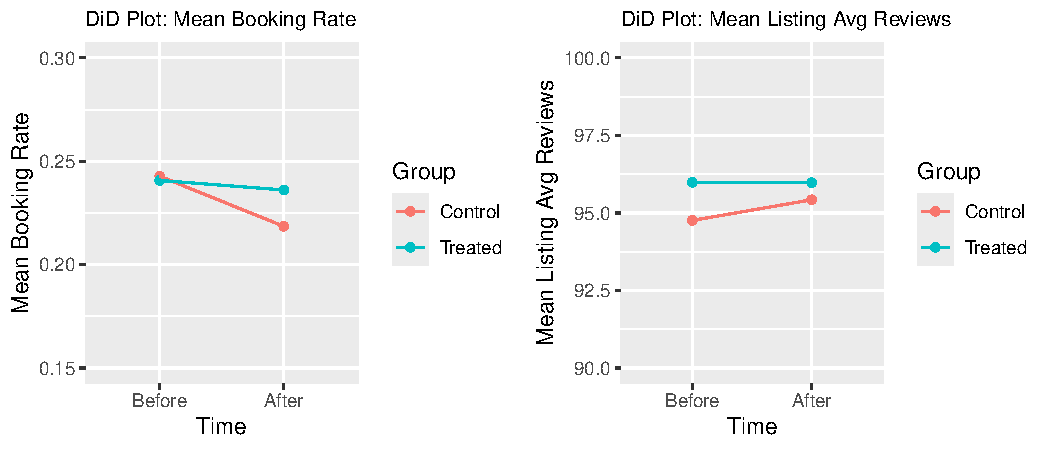
\includegraphics{assignment2_final_2_files/figure-latex/unnamed-chunk-15-1.pdf}

The line graphs show the trends over time for booking rates and average
review ratings. The first graph highlights a divergence in booking rates
where treated cities stabilize while control cities decline. The graph
for the average reviews shows the opposite as the gap between the two
groups is narrowing. Together, these visualizations suggest that the
Airbnb Plus program's impact is more noticeable in stabilizing booking
rates than in influencing average reviews.

\section{3. Regression Analysis: Estimating the Impact of Airbnb
Plus}\label{regression-analysis-estimating-the-impact-of-airbnb-plus}

In this section, we apply regression analysis to estimate the impact of
the Airbnb Plus program, controlling for city-specific factors using
fixed city effects. By incorporating fixed effects, we account for
unobserved heterogeneity across cities that could influence the outcome
variables, such as booking rate and average reviews. This approach helps
isolate the effect of Airbnb Plus from other city-level influences,
providing a more robust estimation of the program's impact. The Fixed
Effects results for \textbf{booking\_rates} show that the Plus program
has a marginally significant effect on booking rates for treated cities
after its implementation. After including control variables, the
interaction term loses its significance, meaning that the Plus program's
effect on booking rates may be explained by factors like property
characteristics (\emph{year\_built\_to\_now}) or specific rental market
conditions (\emph{log\_price\_mean}), rather than the program itself.
For instance, it can be observed that for every unit increase in
\emph{price\_mean}, \emph{booking\_rate} decreases by 0.023 units, while
every unit increase in \emph{year\_built\_to\_now} leads to 0.01 pp
increase in \emph{booking\_rate}. Ultimately, there is no evidence that
the interaction effect is different from zero, so we \textbf{fail to
reject} the null hypothesis. The Fixed Effects results for
\textbf{listing\_avg\_reviews} show a \textbf{significantly negative}
interaction term before and after including the control variables.
Contrary to expectations, the Plus program may have had an adverse
effect on average reviews in treated cities, potentially due to
unintended consequences or negative customer experiences associated with
the program. The observed effect seems to not be driven by confounding
factors, such as differences in listing characteristics
(\emph{log\_price\_mean} or \emph{year\_built\_to\_now}) or economic
conditions (\emph{employment\_rate}). Since the interaction term is
statistically different from zero, we \textbf{fail to reject} the null
hypothesis. The control variables provide further insights into factors
influencing listing average reviews. For every unit increase in
\emph{price\_mean}, listing average reviews increase by 0.75 units,
suggesting that higher prices may be associated with higher perceived
quality or guest satisfaction. For every unit increase in
\emph{year\_built\_to\_now} (indicating older properties), listing
average reviews decrease by 0.025 units, possibly reflecting a
preference for older, more established properties. For every unit
increase in \emph{employment\_rate}, listing average reviews increase by
14.8 units, highlighting the potential influence of local economic
conditions on guest experiences. While the Plus program might not have
achieved its intended effects, other property and market characteristics
play a significant role in shaping outcomes.

\begin{table}[!htbp] \centering 
  \caption{Fixed Effects Regression Results} 
  \label{} 
\tiny 
\begin{tabular}{@{\extracolsep{5pt}}lcccc} 
\\[-1.8ex]\hline 
\hline \\[-1.8ex] 
 & \multicolumn{4}{c}{\textit{Dependent variable:}} \\ 
\cline{2-5} 
\\[-1.8ex] & \multicolumn{2}{c}{Booking Rate} & \multicolumn{2}{c}{Listing Avg Review} \\ 
 & BR (no controls) & BR (with controls) & LAR (no controls) & LAR (with controls) \\ 
\\[-1.8ex] & (1) & (2) & (3) & (4)\\ 
\hline \\[-1.8ex] 
 timeAfter & $-$0.024$^{***}$ & $-$0.015$^{***}$ & 0.665$^{***}$ & 0.314$^{***}$ \\ 
  & (0.002) & (0.002) & (0.045) & (0.041) \\ 
  employment\_rate &  & 0.009 &  & 14.891$^{***}$ \\ 
  &  & (0.038) &  & (0.689) \\ 
  log\_price\_mean &  & $-$0.023$^{***}$ &  & 0.752$^{***}$ \\ 
  &  & (0.002) &  & (0.042) \\ 
  year\_built\_to\_now &  & 0.001$^{***}$ &  & $-$0.025$^{***}$ \\ 
  &  & (0.0001) &  & (0.001) \\ 
  timeAfter:groupTreated & 0.010$^{*}$ & 0.003 & $-$0.768$^{***}$ & $-$0.524$^{***}$ \\ 
  & (0.005) & (0.005) & (0.106) & (0.095) \\ 
 \hline \\[-1.8ex] 
Observations & 10,702 & 10,702 & 10,702 & 10,702 \\ 
R$^{2}$ & 0.011 & 0.080 & 0.020 & 0.227 \\ 
Adjusted R$^{2}$ & 0.011 & 0.080 & 0.020 & 0.226 \\ 
F Statistic & 61.482$^{***}$ (df = 2; 10695) & 187.090$^{***}$ (df = 5; 10692) & 109.945$^{***}$ (df = 2; 10695) & 626.761$^{***}$ (df = 5; 10692) \\ 
\hline 
\hline \\[-1.8ex] 
\textit{Note:}  & \multicolumn{4}{r}{$^{*}$p$<$0.1; $^{**}$p$<$0.05; $^{***}$p$<$0.01} \\ 
\end{tabular} 
\end{table}

\section{4. Assumptions and Model
Diagnostics}\label{assumptions-and-model-diagnostics}

\subsubsection{1. Linearity}\label{linearity}

For the scope of this research, linearity of the panel data model was
assumed. Future work should assess linearity to validate model
assumptions, though achieving it may be challenging due to demographic
and economic variability across cities.

\subsubsection{2. Random Sampling}\label{random-sampling}

The non-random selection of treated cities, geographic bias, and
staggered program implementation challenge the random sampling
assumption. Efforts to address this included imputing missing data,
treating outliers in listing\_avg\_review and employment\_rate,
truncating booking\_rate and reviews at the 5th and 95th percentiles,
and log-transforming price\_mean, but significant biases likely remain.

\subsubsection{3. Multicollinearity}\label{multicollinearity}

While no severe multicollinearity issues are evident, moderate
correlations (year\_built\_to\_now and listing\_avg\_review vs.~zipcode)
may still affect the model's interpretation. The Variance Inflation
Factor (VIF) diagnostics confirm this assumption was not violated as all
VIF results are below 5, indicating low predictors' multicollinearity.

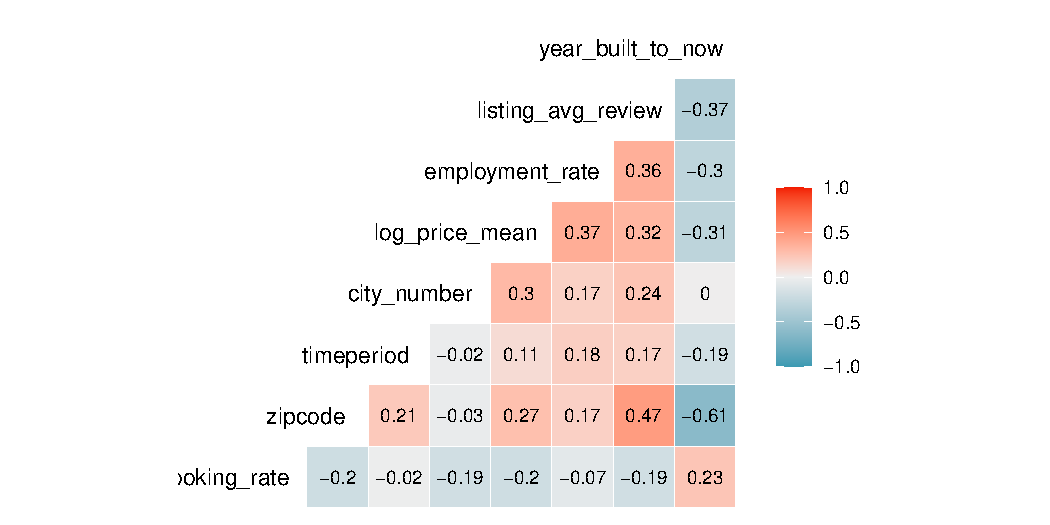
\includegraphics{assignment2_final_2_files/figure-latex/unnamed-chunk-17-1.pdf}

\subsubsection{4. Zero conditional mean}\label{zero-conditional-mean}

The assumption of zero conditional mean is challenged by omitted
variable bias, as unobserved factors likely influence booking rates and
average reviews beyond the study's scope. Potential measurement errors
were noted in \textbf{employment\_rate}, which may not reflect monthly
fluctuations; \textbf{price\_mean}, affected by price volatility and
promotions; and \textbf{year\_built\_to\_now}, susceptible to inaccurate
or misreported property records. Simultaneity is also a concern, as
dependent variables like booking rates and reviews may influence
independent factors such as employment, housing construction, and
pricing. These issues highlight the complexity of fully isolating causal
relationships in this analysis.

\subsubsection{5. Homoscedasticity}\label{homoscedasticity}

The studentized Breusch-Pagan test checks if the error term has the same
variance given any values of the explanatory variable. The results of
the test showed very small p-values for all models, indicating a
violation of the homoscedasticity assumption. This violation can be
attributed to inherent differences between cities, such as variations in
population size, economic conditions, tourism activity, and other
contextual factors.

\subsubsection{6. Normality of Residuals}\label{normality-of-residuals}

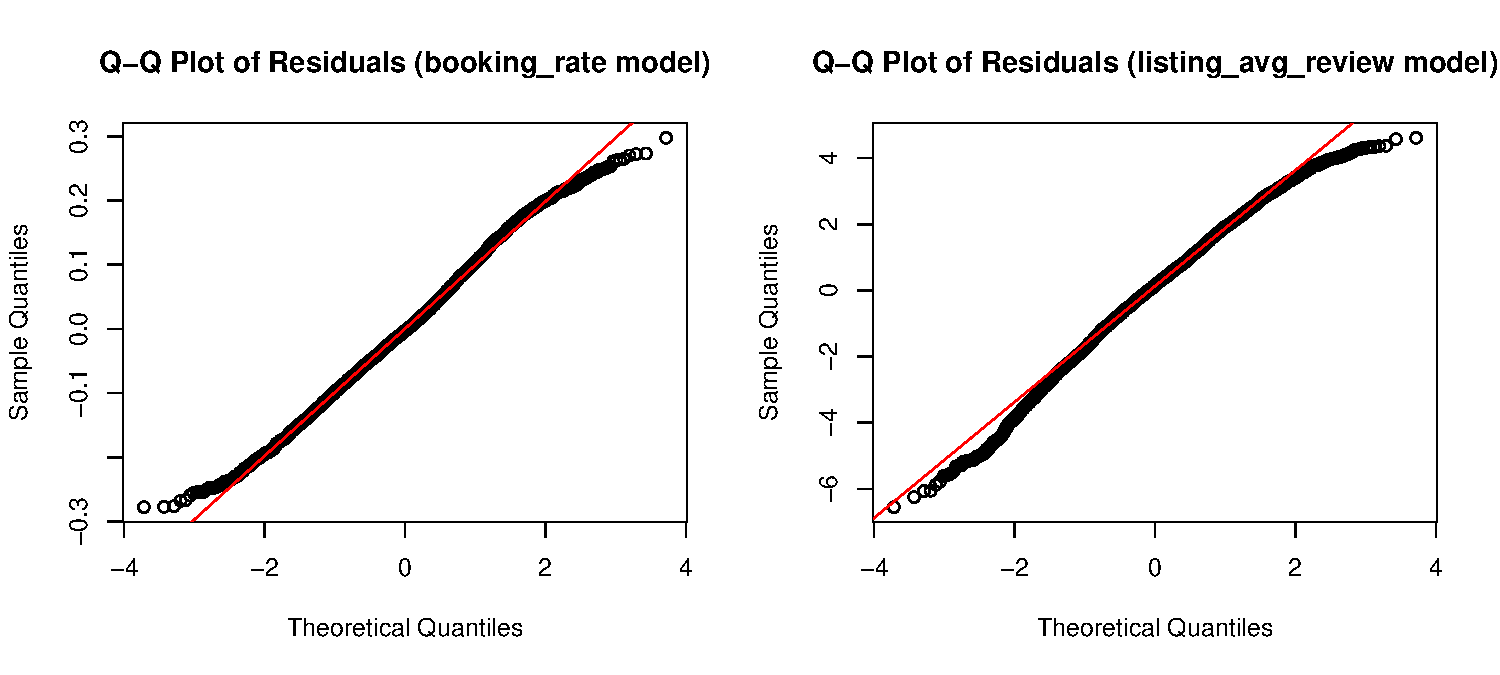
\includegraphics{assignment2_final_2_files/figure-latex/unnamed-chunk-20-1.pdf}
The Q-Q plots for both models, booking\_rate and listing\_avg\_review,
show that the residuals in the central area (approx. between -2.5 and
+2) are close to the normal distribution. In the extreme areas, the
points deviate slightly from the line - for very negative values they
are slightly above, for very positive values slightly below. Such
deviations are common in large samples and hardly affect the analysis.
The Shapiro-Wilk tests resulted in very small p-values (p \textless{}
0.0001), which indicates statistically significant deviations from the
normal distribution. However, the W values are close to 1 (0.99688 for
booking\_rate and 0.99342 for listing\_avg\_review), which means a good
approximation to the normal distribution. Significant p-values are to be
expected for large samples, as the test is very sensitive to small
deviations. The normality assumption of the residuals is fulfilled in
the central area, where the majority of the data lies. The slight
deviations in the extreme ranges are tolerable and do not significantly
affect the estimates of the regression coefficients or the statistical
inference. Overall, the models are reliable and the results remain
valid.

\section{5. Discussion and Business
Implications}\label{discussion-and-business-implications}

This study examined the impact of the Airbnb Plus program on booking
rates and customer satisfaction across various U.S. cities. The analysis
revealed no statistically significant impact of the program on booking
rates in treated cities compared to control cities. While treated cities
experienced stabilization in booking rates, these changes appear to be
driven more by external factors such as market conditions and property
characteristics than the introduction of the Plus program itself.
Interestingly, the program was associated with a slight decrease in
average reviews, suggesting potential mismatches between customer
expectations and actual experiences. Higher pricing for Plus-certified
listings likely led to elevated customer expectations, making them more
critical in reviews when expectations were unmet. Higher prices
negatively influenced booking rates, which is in line with business
expectations. However, higher prices correlated with improved customer
satisfaction, possibly due to better property matching and higher
quality expectations. Older buildings tended to have higher booking
rates, possibly reflecting unique charm or historical value. Conversely,
these older properties were associated with lower customer satisfaction,
potentially due to reliability or maintenance issues. Cities with higher
employment rates showed significantly higher booking rates, indicating
economic factors play a critical role in driving demand. This study
faced several limitations, including potential non-linear relationships
in the data, geographic and temporal biases from the non-random
selection of treated cities, and omitted variable bias due to unobserved
factors affecting booking rates and customer satisfaction. Measurement
errors in variables such as employment rate and average price, as well
as heteroscedasticity caused by city-specific variations, further
impacted the analysis. However, residuals closely approximated normality
in the central ranges, enhancing the reliability of the regression
coefficients and statistical inferences. Future research could address
these limitations by exploring non-linear modeling techniques and
accounting for more unobserved factors to improve explanatory power.
However, building on previous research, this study concludes that the
Airbnb Plus program is not a worthy investment for the company. If
further research on the topic were to be conducted, this study suggests
exploring the impact of booking rates across each treated city,
highlighting which socio-economic and seasonal factors enhance the
program's success. By doing so, the program could be implemented only in
cities that meet these requirements, thereby boosting Airbnb's revenue.
These cities are expected to be large central business districts (CBDs)
with high employment rates, relatively low listing prices, and a good
number of historical buildings.

\section{Disclaimer}\label{disclaimer}

This research paper had its code deliberately debugged with the help of
AI, making sure that the inevitable human errors were swiftly corrected
by our digital assistant. Rest assured, no robots were harmed in the
process, and the human touch remained essential. Other than debugging,
AI was also used for coding suggestions and alternatives.

\end{document}
